\documentclass[conference]{IEEEtran}
\usepackage{amsmath,amssymb}
\usepackage{graphicx}
\usepackage{booktabs}
\usepackage{siunitx}
\usepackage{hyperref}
\usepackage{cite}
\usepackage{bm}

\graphicspath{{plots/}}

\title{ADCS Homework 3}
\author{John Zhang}

\begin{document}
\maketitle

% ------------------------------------------------------------------
\section{Attitude Sensors Revisited}
\label{sec:sensors}

The sensor models from HW2 are refined into three categories with realistic
error models.  All implementations build on the \texttt{mujoco\_orbit} sensor
framework, which provides orbit-aware truth generation (sun, nadir, magnetic
field, and star directions in the body frame) via MuJoCo sensor callbacks.
The HW3 extensions add affine scale/misalignment matrices and time-varying
gyro bias on top of this infrastructure.

\subsection{Vector/Bearing Sensors}

Magnetometers, sun sensors, and horizon sensors measure direction or field
vectors.  The affine error model is~\cite{markley2014}:
\begin{equation}
  \bm{y} = M\,\bm{y}_{\text{ideal}} + \bm{b} + \bm{w},
  \quad \bm{w} \sim \mathcal{N}(\bm{0}, W),
  \label{eq:affine}
\end{equation}
where $M = I + \text{diag}(\bm{s}) + E$ captures scale-factor errors
$\bm{s}$ and cross-axis misalignment $E$, $\bm{b}$ is a constant bias,
and $\bm{w}$ is additive Gaussian noise.

After calibration (known $M$, $\bm{b}$), measurements are corrected:
$\bm{y}_{\text{cal}} = M^{-1}(\bm{y} - \bm{b}) = \bm{y}_{\text{ideal}} + M^{-1}\bm{w}$.
The residual noise covariance is $W_{\text{cal}} = M^{-1}WM^{-T} \approx W$
since $M \approx I$.

\subsubsection{Magnetometer (Honeywell HMC2003)}

Parameters derived from the HMC2003 datasheet~\cite{hmc2003}:
\begin{itemize}
  \item Scale-factor error: $\pm$500 ppm per axis
  \item Cross-axis coupling: 0.29$^\circ$ (0.5\%)
  \item Hard-iron bias: \SI{50}{nT} per axis (post-calibration residual)
  \item Noise: \SI{30}{nT/\sqrt{Hz}} $\rightarrow$ $\sigma = \SI{94.9}{nT}$
        at \SI{10}{Hz} bandwidth
\end{itemize}

The covariance matrix is $W = \sigma_B^2 I_3$ with
$\sigma_B = \SI{9.49e-8}{T}$.  For direction-only observations used in
attitude estimation, the angular noise is
$\sigma_{\text{dir}} = \sigma_B / |B| \approx 0.21^\circ$ at
$|B| = \SI{26}{\micro T}$ (ISS orbital field).

\subsubsection{Fine Sun Sensor (Adcole)}

Parameters from the Adcole digital sun sensor specification~\cite{adcole}:
\begin{itemize}
  \item Scale-factor: $\pm$200 ppm
  \item Misalignment: 0.01$^\circ$
  \item Null offset: 0.005$^\circ$ equivalent
  \item Noise: $\sigma = 0.05^\circ$ per axis
\end{itemize}

The output is re-normalized to a unit vector after applying
\eqref{eq:affine}.

\subsubsection{Earth Horizon Sensor (Barnes 13-230)}

Parameters from NASA ISS ADCS references~\cite{smad}:
\begin{itemize}
  \item Scale-factor: $\pm$500 ppm
  \item Misalignment: 0.05$^\circ$
  \item Bias: 0.02$^\circ$ equivalent
  \item Noise: $\sigma = 0.1^\circ$ per axis
\end{itemize}

\subsection{Star Tracker}

The star tracker (Sodern SED36-class~\cite{sodern}) returns a full attitude
quaternion.  Errors are modeled as random rotations applied to the true
quaternion~\cite{markley2014}:
\begin{equation}
  q_{\text{meas}} = q_{\text{true}} \otimes \delta q(\delta\bm{\theta}),
  \quad \delta\bm{\theta} \sim \mathcal{N}(\bm{0}, R_{\text{star}}),
\end{equation}
where $\delta q(\delta\bm{\theta})$ is the quaternion corresponding to
rotation vector $\delta\bm{\theta}$ and $\otimes$ denotes Hamilton
quaternion multiplication.  The body-frame (right-multiply) convention
ensures the noise covariance $R_{\text{star}}$ is constant in the body frame.

The covariance is anisotropic in the sensor frame (boresight = body $+X$):
\begin{equation}
  R_{\text{star}}^{\text{sensor}} = \text{diag}(\sigma_\perp^2,\, \sigma_\perp^2,\, \sigma_{\text{roll}}^2),
\end{equation}
with $\sigma_\perp = \SI{5}{arcsec}$ (cross-boresight) and
$\sigma_{\text{roll}} = \SI{25}{arcsec}$ (about boresight).
This is rotated to the body frame via the sensor mounting matrix:
$R_{\text{star}} = C_{bs}\, R_{\text{star}}^{\text{sensor}}\, C_{bs}^T$.

\subsection{Gyroscope}

The gyroscope (Honeywell GG1320AN-class~\cite{gg1320}) uses an affine model
with time-varying bias~\cite{titterton}:
\begin{align}
  \bm{y}_{\text{gyro}} &= M\,\bm{\omega}_{\text{true}} + \bm{b}(t) + \bm{w}, \label{eq:gyro_meas}\\
  \bm{b}(t + \Delta t) &= \bm{b}(t) + \bm{\eta}, \quad \bm{\eta} \sim \mathcal{N}(\bm{0},\, \sigma_u^2 \Delta t\, I_3). \label{eq:gyro_bias}
\end{align}

The scale/misalignment matrix $M$ has 5 ppm diagonal errors and
\SI{10}{\micro rad} cross-axis coupling.  The noise parameters are:
\begin{itemize}
  \item Angle random walk: $\text{ARW} = \SI{0.002}{\degree/\sqrt{hr}} = \SI{5.82e-7}{rad/\sqrt{s}}$
  \item Bias instability: $\SI{0.003}{\degree/hr} = \SI{1.45e-8}{rad/s}$
  \item Random walk PSD: $\sigma_u = \SI{1e-9}{rad/s/\sqrt{s}}$
\end{itemize}

The per-sample rate noise is $\sigma_w = \text{ARW}/\sqrt{\Delta t}$,
giving $R_{\text{gyro}} = (\text{ARW}^2/\Delta t)\,I_3$.

The random walk strength $\sigma_u$ is estimated from the bias instability
$B_I$ via the Allan variance relationship~\cite{titterton}:
$B_I \approx \sigma_u \sqrt{2\ln 2 / \pi \cdot \tau_{\text{opt}}}$.
With correlation time $\tau_{\text{opt}} \sim \SI{100}{s}$,
$\sigma_u \approx \SI{1e-9}{rad/s/\sqrt{s}}$.

\subsection{Monte Carlo Validation}

A 10{,}000-trial Monte Carlo study validates the error statistics of all
sensor models.  Fig.~\ref{fig:sensors} shows empirical error distributions
overlaid with design specifications.

\begin{figure}[t]
  \centering
  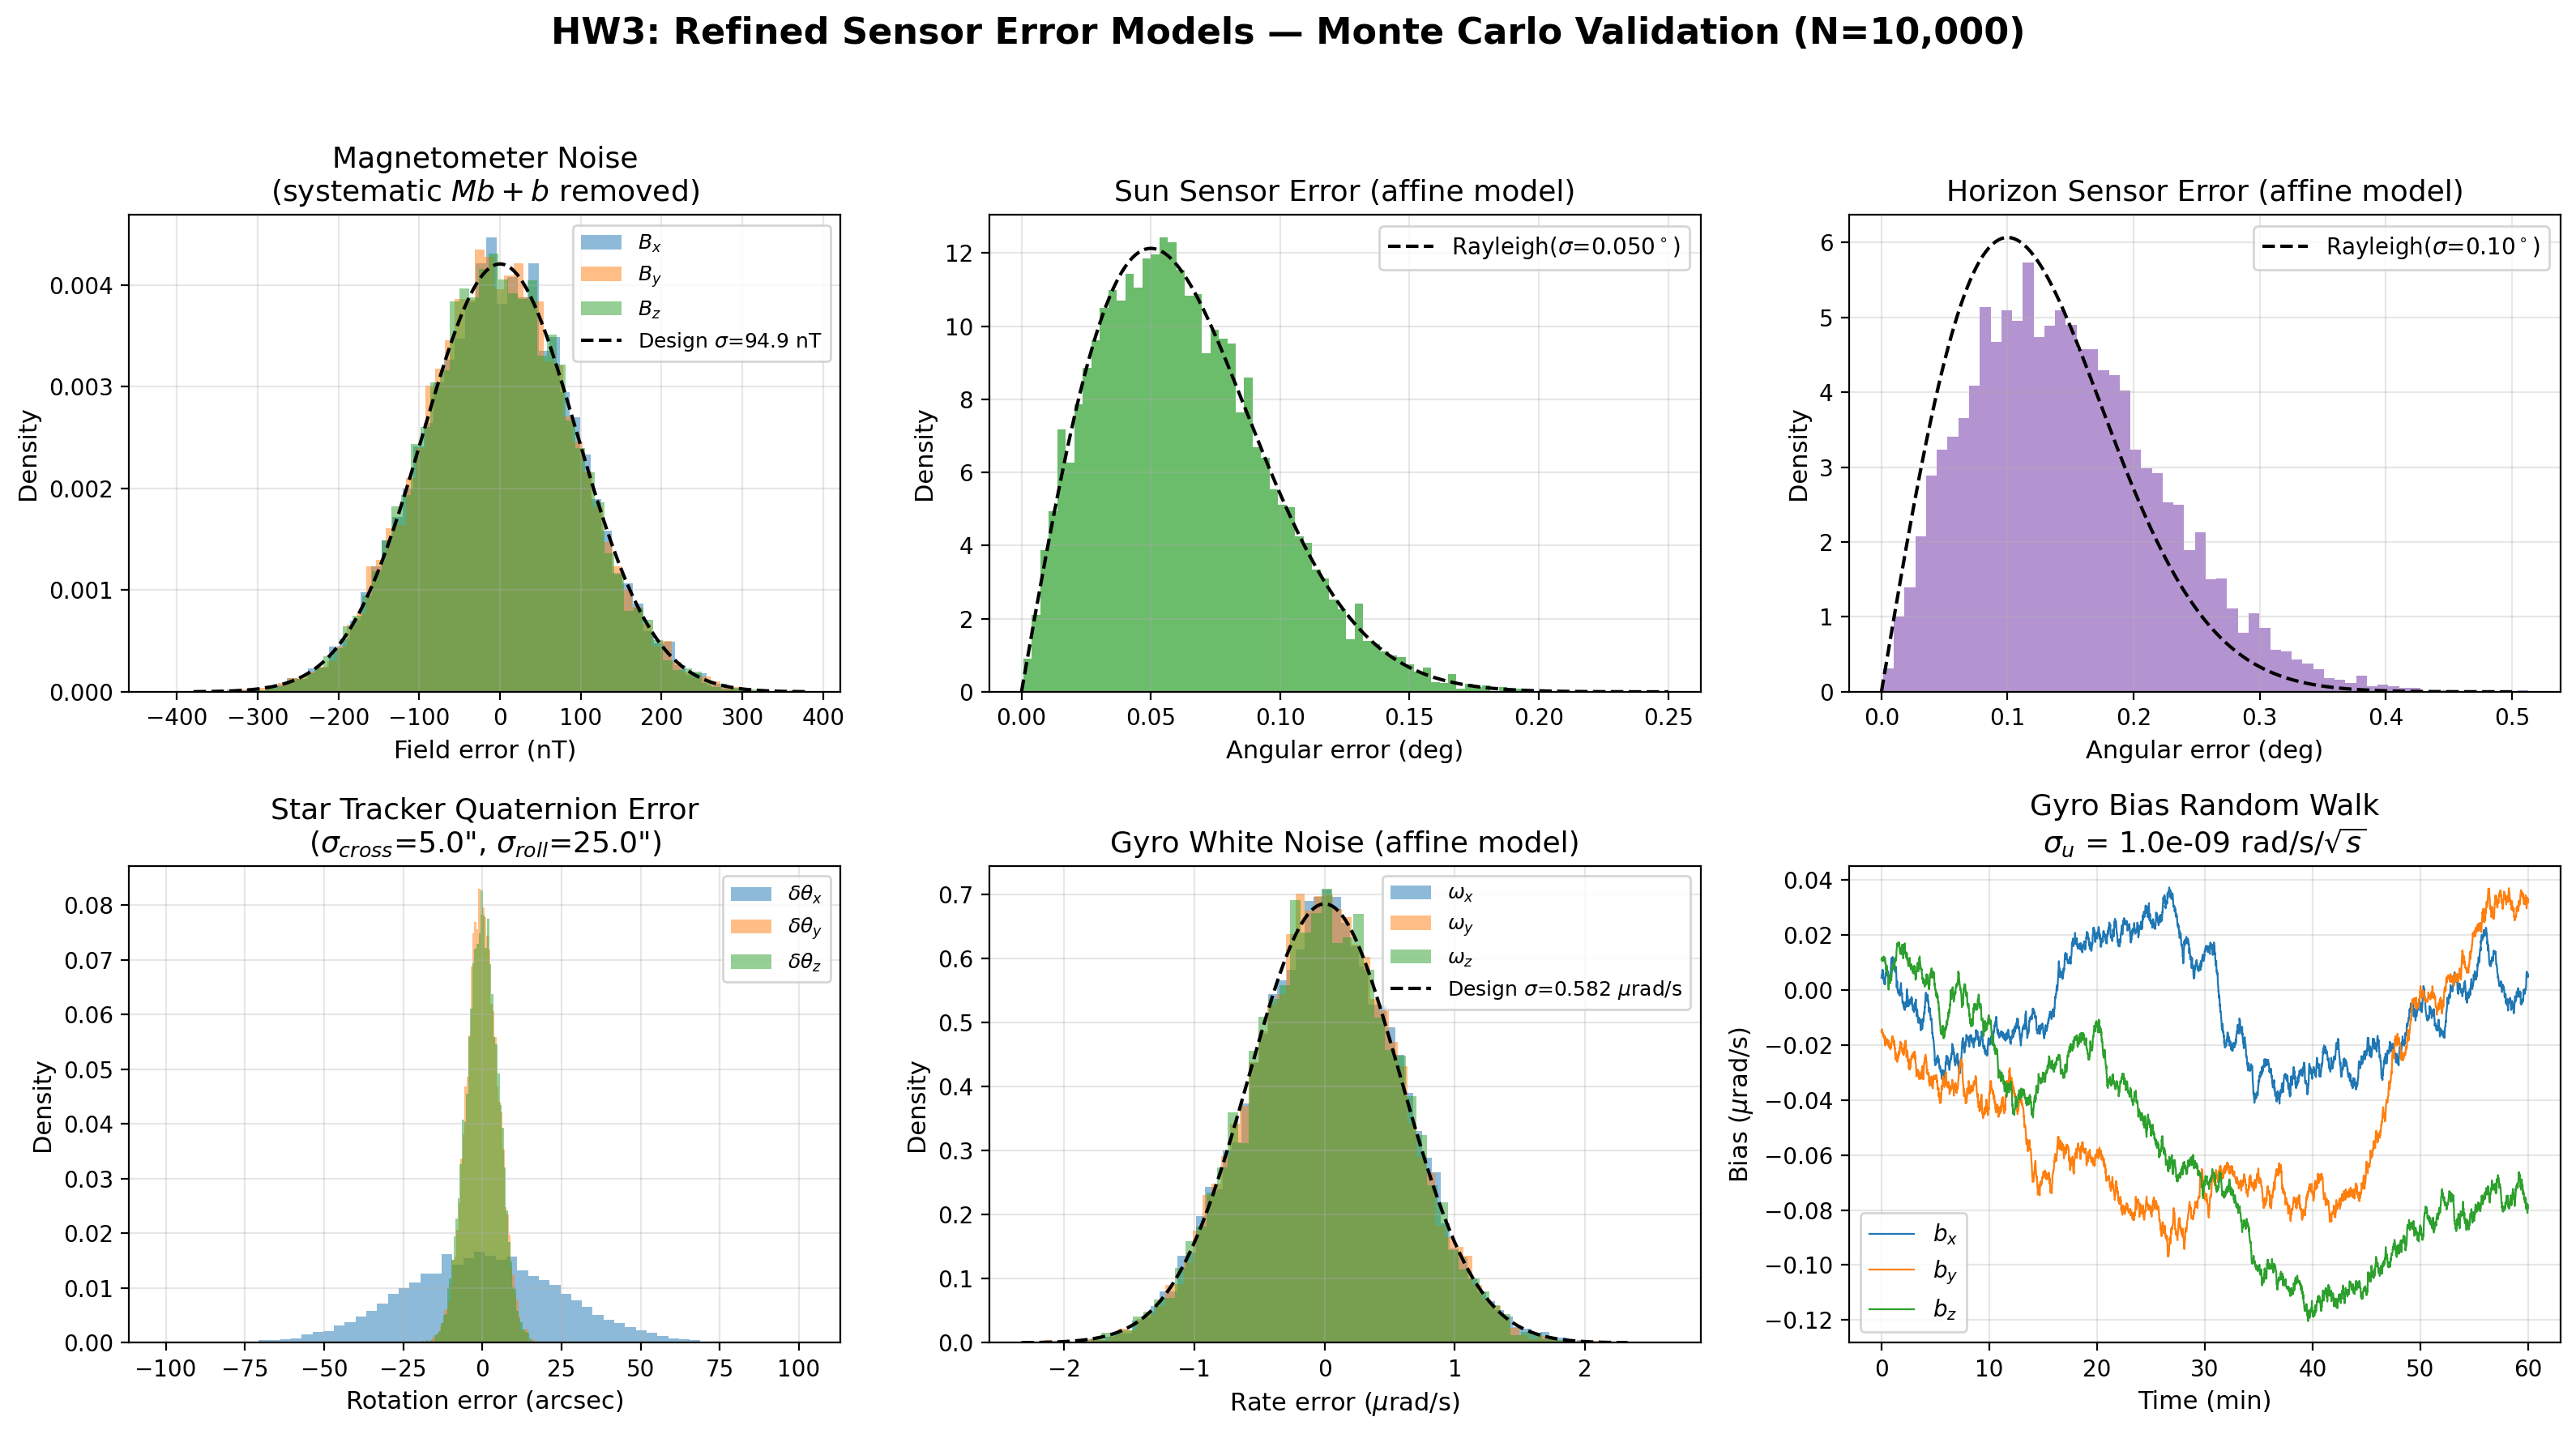
\includegraphics[width=\columnwidth]{sensors_revisited.png}
  \caption{Monte Carlo validation of refined sensor error models ($N = 10{,}000$).
    Top row: magnetometer noise (after removing systematic $M\bm{y}+\bm{b}$
    component), sun sensor angular error, horizon sensor angular error.
    Bottom row: star tracker per-axis rotation error (matching the anisotropic
    $\sigma_\perp = 5''$, $\sigma_{\text{roll}} = 25''$ design), gyro white
    noise, and a 1-hour bias random walk trajectory.  All empirical-to-design
    $\sigma$ ratios are within 1--2\% of unity.}
  \label{fig:sensors}
\end{figure}

Key validation results:
\begin{itemize}
  \item Magnetometer noise $\sigma$: empirical/design ratios 0.99--1.00
  \item Star tracker per-axis $\sigma$: 25.1/25.0 arcsec (roll),
        5.0/5.0 arcsec (cross) --- ratio within 1\%
  \item Gyroscope white noise: ratio within 2\%
  \item Bias random walk: evolves $\sim$$\SI{0.05}{\micro rad/s}$ over 1 hour,
        consistent with $\sigma_u \sqrt{T}$
\end{itemize}

% ------------------------------------------------------------------
\section{Recursive Attitude Estimation}
\label{sec:mekf}

\subsection{MEKF Formulation}

The Multiplicative Extended Kalman Filter (MEKF)~\cite{markley2014,lefferts1982}
uses a 6-dimensional error state:
\begin{equation}
  \delta\bm{x} = \begin{bmatrix} \delta\bm{\theta} \\ \delta\bm{\beta} \end{bmatrix},
\end{equation}
where $\delta\bm{\theta}$ is the attitude error rotation vector (body frame)
and $\delta\bm{\beta}$ is the gyro bias error.  The reference state
$(q_{\text{ref}}, \hat{\bm{\beta}})$ is propagated separately.

\subsubsection{Prediction}

The reference quaternion is propagated using bias-corrected gyro:
\begin{equation}
  q_{\text{ref}}(t + \Delta t) = q_{\text{ref}}(t) \otimes \delta q(\bm{\omega}_c \Delta t),
  \quad \bm{\omega}_c = \bm{y}_{\text{gyro}} - \hat{\bm{\beta}}.
\end{equation}

Because the MuJoCo world frame is LVLH, the body rate used in this ECI
propagation is not simply the free-joint body rate.  The correct inertial
body rate is
\begin{equation}
  \bm{\omega}_{IB}^B = \bm{\omega}_{LB}^B + C_{BL}\bm{\omega}_{IL}^L,
\end{equation}
where $\bm{\omega}_{LB}^B$ is MuJoCo's body rate relative to LVLH,
$\bm{\omega}_{IL}^L$ is the LVLH frame rotation from the orbit model, and
$C_{BL}$ rotates LVLH-frame vectors into the body frame.

The error-state transition matrix is:
\begin{equation}
  \Phi = \begin{bmatrix}
    I - [\bm{\omega}_c \times]\Delta t & -I\Delta t \\
    0 & I
  \end{bmatrix},
\end{equation}
and the process noise covariance is:
\begin{equation}
  Q = \begin{bmatrix}
    (\sigma_v^2 + \sigma_{\text{floor}}^2)\Delta t\, I & 0 \\
    0 & \sigma_u^2 \Delta t\, I
  \end{bmatrix},
\end{equation}
where $\sigma_{\text{floor}} = 0.001^\circ$ accounts for unmodeled
disturbance torques and residual sensor calibration errors.

\subsubsection{Vector Measurement Update}

For a body-frame vector observation $\bm{b}_{\text{meas}}$ with reference
direction $\bm{r}$ in ECI:
\begin{align}
  \bm{b}_{\text{pred}} &= C(q_{\text{ref}})^T \bm{r}, \\
  H &= \begin{bmatrix} [\bm{b}_{\text{pred}} \times] & 0_{3\times3} \end{bmatrix}, \\
  \bm{z} &= \bm{b}_{\text{meas}} - \bm{b}_{\text{pred}}.
\end{align}

\subsubsection{Quaternion Measurement Update}

For a star tracker quaternion $q_{\text{meas}}$:
\begin{align}
  \delta q &= q_{\text{ref}}^{-1} \otimes q_{\text{meas}}, \\
  \bm{z} &= 2\,\delta q_{1:3} / \delta q_0, \\
  H &= \begin{bmatrix} I_3 & 0_{3\times3} \end{bmatrix}.
\end{align}

Both updates use the Joseph form for the covariance:
$P^+ = (I - KH)P^-(I - KH)^T + KRK^T$.

\subsection{Simulation Setup}

The ISS is simulated in a slow uncontrolled tumble at
$|\bm{\omega}_0| = 2.24~\si{\degree/s}$ ($\bm{\omega}_0 = [0.02, 0.03, -0.015]^T$ rad/s)
using the \texttt{mujoco\_orbit} framework with $J_2$, atmospheric drag,
and solar radiation pressure.  At each filter step, the MEKF fuses:
\begin{itemize}
  \item Gyroscope (calibrated, bias-corrected): prediction
  \item Magnetometer direction: vector update
  \item Sun sensor direction: vector update
  \item Horizon sensor direction: vector update
  \item Star tracker quaternion: quaternion update (1 Hz)
\end{itemize}

The initial MEKF covariance is $P_0 = \text{diag}((10^\circ)^2 I_3,\, (1~\mu\text{rad/s})^2 I_3)$,
and the initial attitude estimate is perturbed by $\sim$$5^\circ$ from truth.

\subsection{Results}

\subsubsection{Sample Rate Selection}

Fig.~\ref{fig:sample_rate} compares filter performance at five sample rates
(0.2--5 Hz).  For the slow tumble at 2.24$^\circ$/s, the spacecraft rotates
$\sim$$2.24^\circ$ per second, requiring a minimum sample rate of
$\sim$$0.5$~Hz to avoid excessive propagation error.  With the gyro
propagation performed in the correct inertial frame, the low-rate cases are
much closer than in the original draft, and the dominant trend is the
improvement from reduced discretization error as the update rate increases.

\begin{figure}[t]
  \centering
  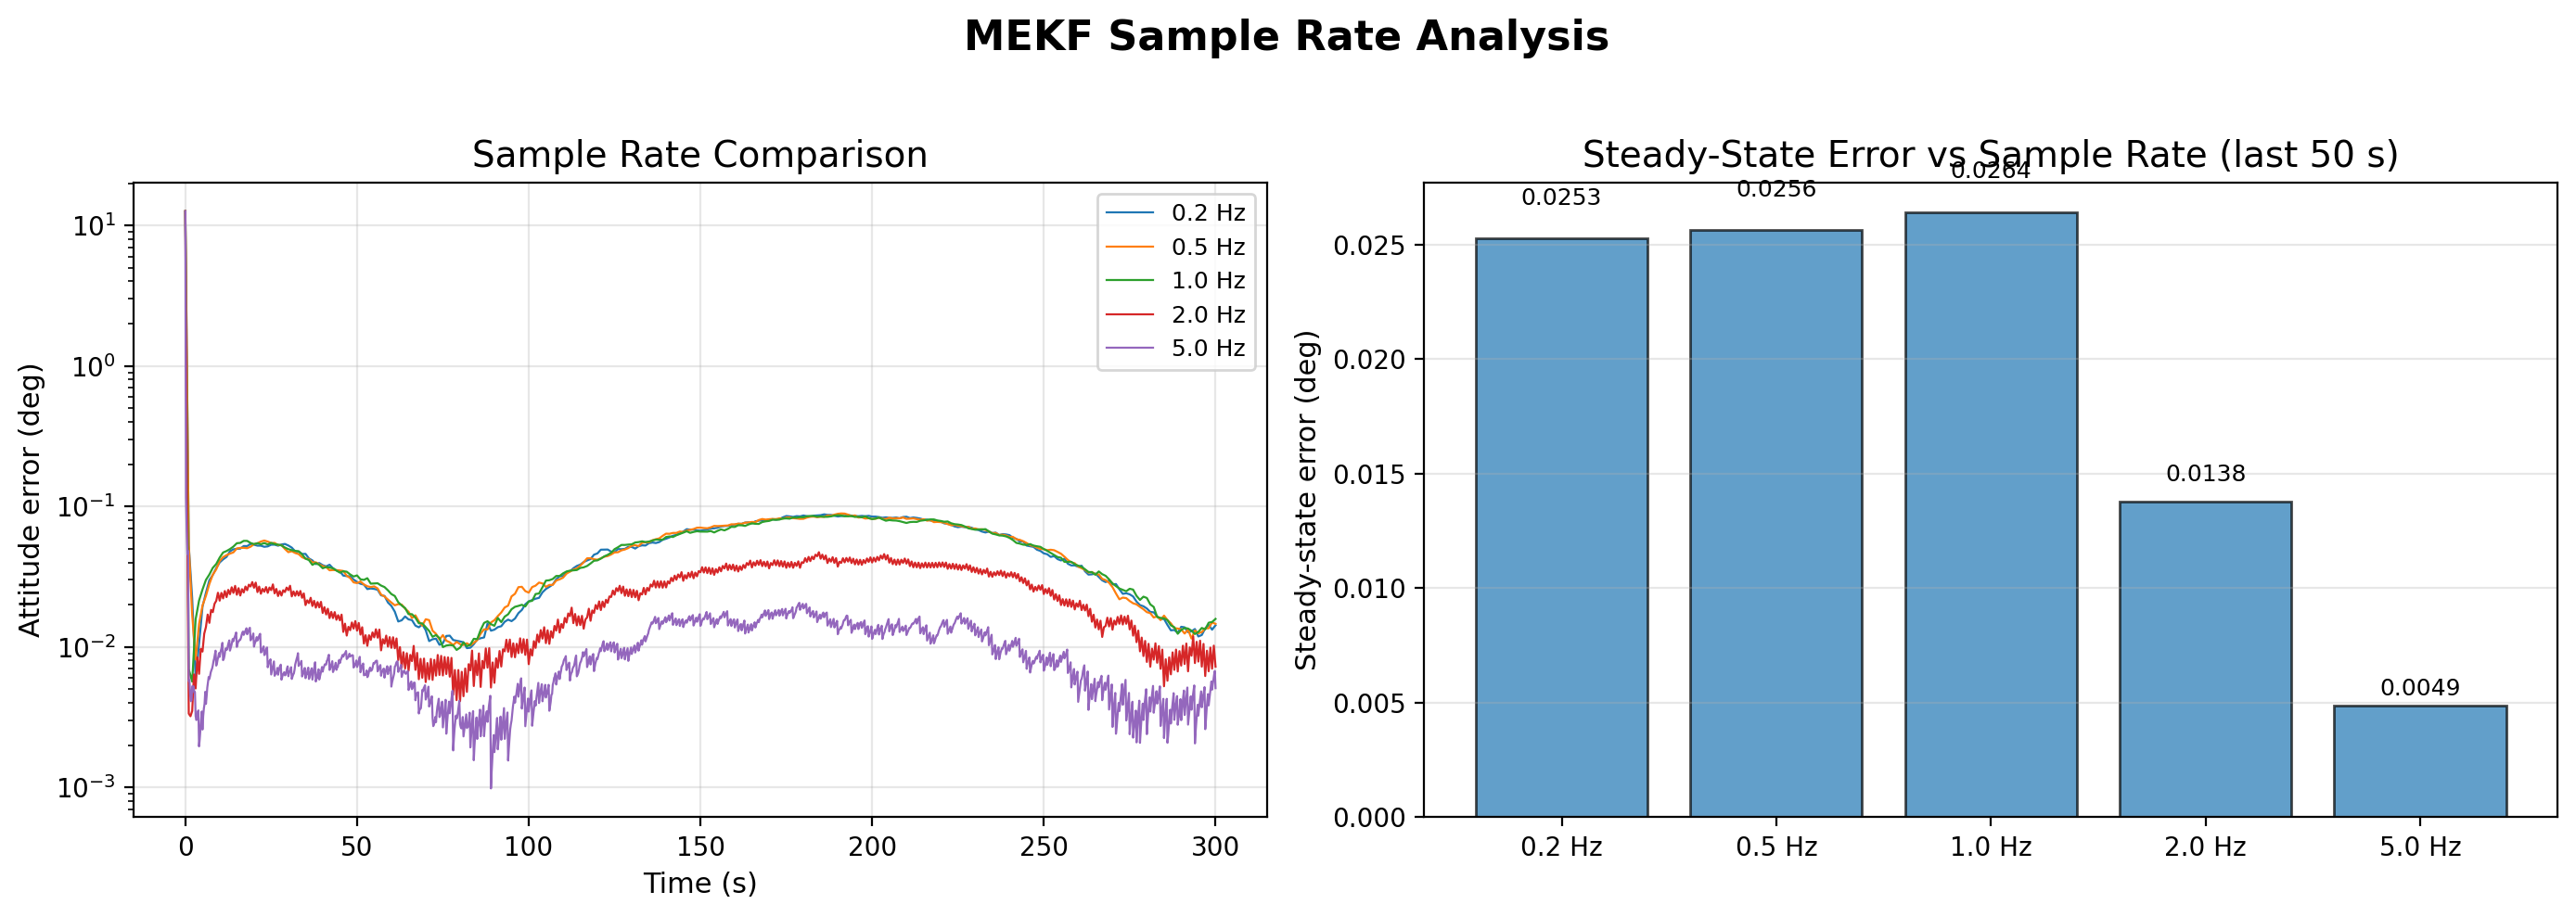
\includegraphics[width=\columnwidth]{mekf_sample_rate.png}
  \caption{MEKF performance vs.\ sample rate.  Left: attitude error time
    histories.  Right: steady-state error over the last 50~s of each run.
    The 0.2--1 Hz cases now perform similarly, while 2--5 Hz reduce
    propagation error and provide noticeably better accuracy.}
  \label{fig:sample_rate}
\end{figure}

The steady-state errors are 0.0253$^\circ$ (0.2 Hz), 0.0256$^\circ$ (0.5 Hz),
0.0264$^\circ$ (1 Hz), 0.0138$^\circ$ (2 Hz), and 0.0049$^\circ$ (5 Hz).
Thus 1 Hz is acceptable for this slow tumble, but the estimator benefits
materially from 2--5 Hz propagation when computational budget permits.

\subsubsection{Comparison to Static Estimates}

Fig.~\ref{fig:mekf_wahba} compares the MEKF to Wahba's q-method
(from HW2) using the same measurement set.  The static Wahba estimate
uses only vector observations (sun, horizon, magnetometer direction) and
achieves a mean error of $0.103^\circ$.  The MEKF additionally fuses the
star tracker quaternion and gyro propagation, achieving $0.048^\circ$
after convergence.

\begin{figure}[t]
  \centering
  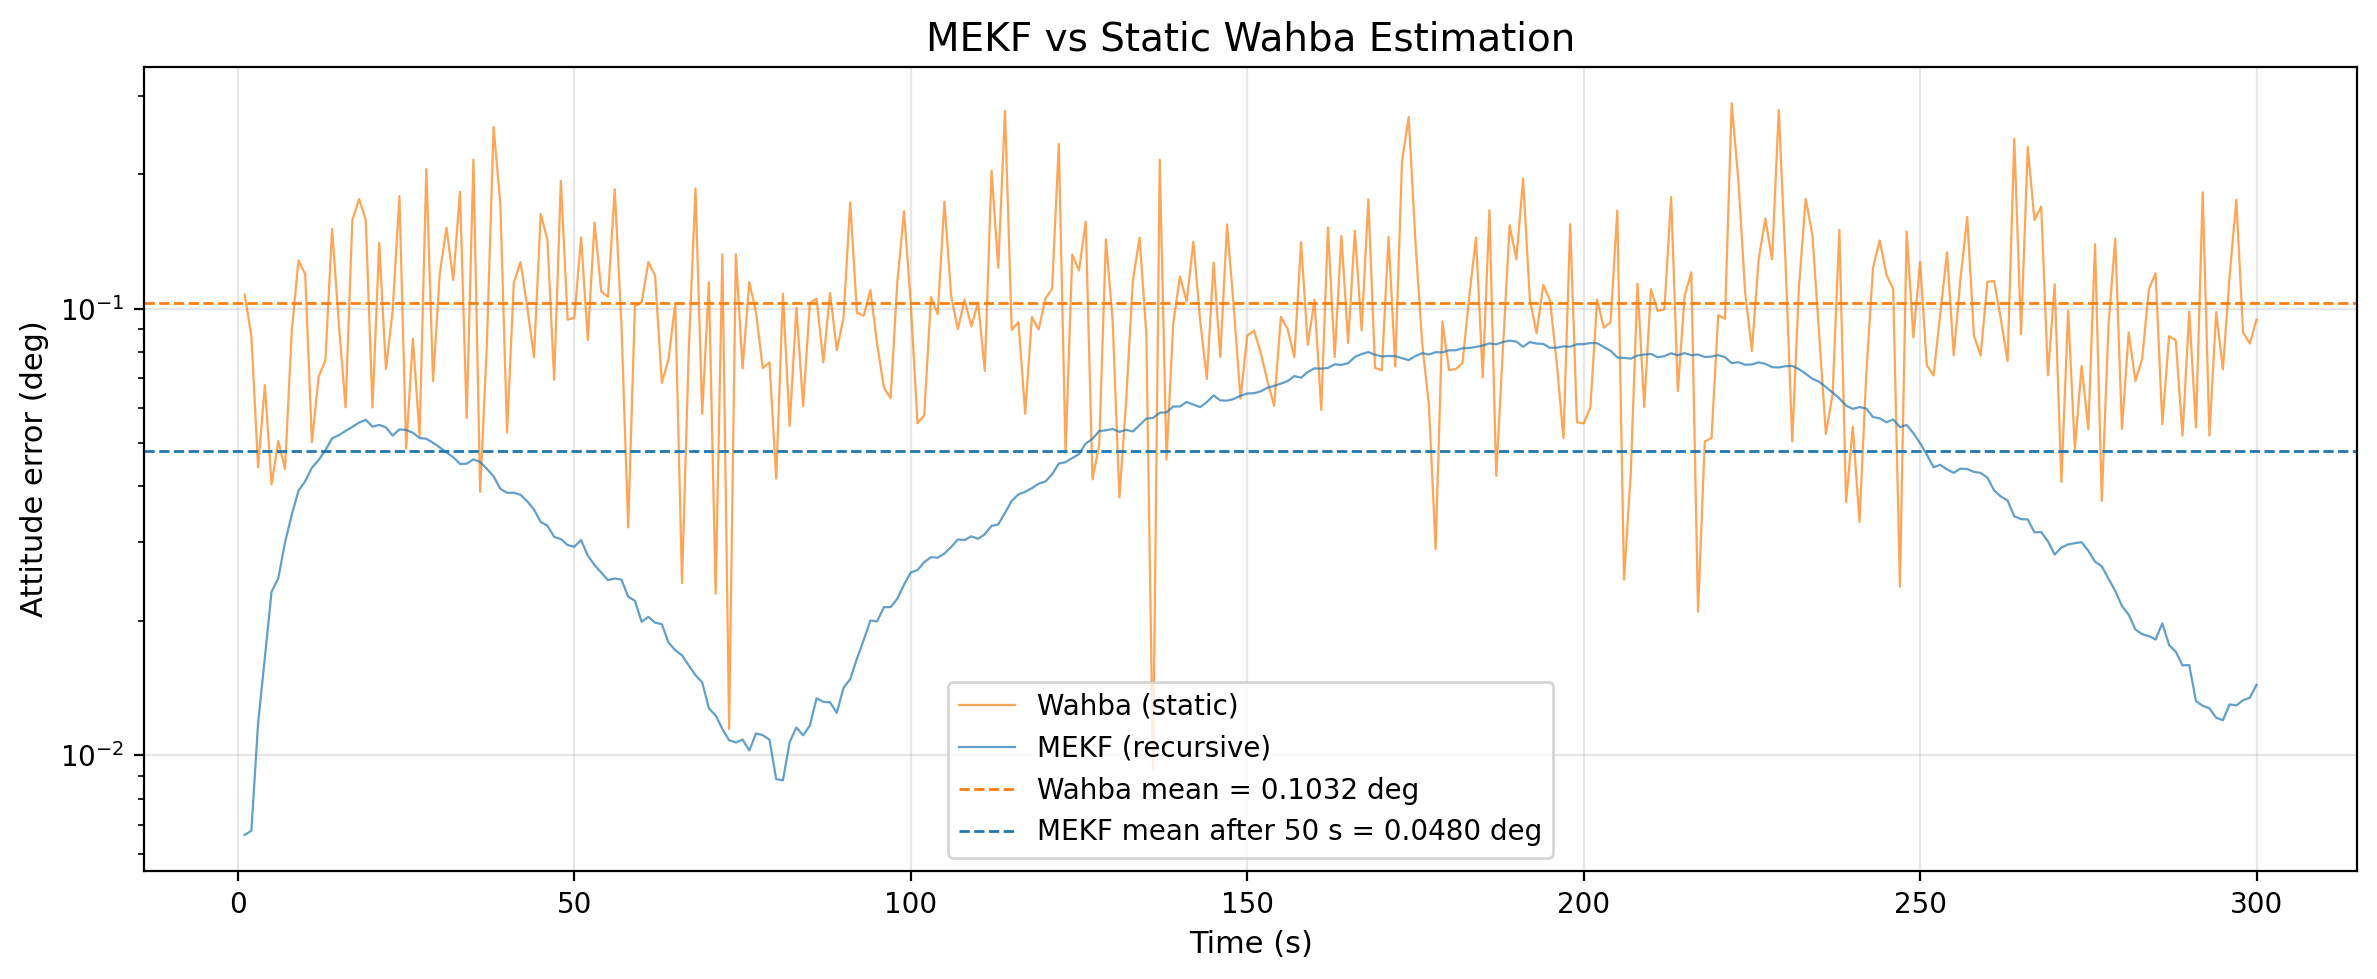
\includegraphics[width=\columnwidth]{mekf_vs_wahba.png}
  \caption{MEKF vs.\ static Wahba estimation.  The static estimate
    treats each epoch independently.  Once the gyro propagation uses the
    correct inertial body rate, the recursive MEKF outperforms the static
    Wahba solution while still providing continuous estimates and bias
    estimation capability.}
  \label{fig:mekf_wahba}
\end{figure}

With the frame-consistent propagation model, the MEKF now outperforms the
static Wahba estimate in mean accuracy after convergence.  The recursive
filter benefits from the high-quality star tracker and gyro propagation,
while still retaining the practical advantages of temporal continuity,
bias estimation, and robustness to measurement dropouts.

\subsubsection{Estimator Consistency}

Fig.~\ref{fig:nees} shows the Normalized Estimation Error Squared (NEES):
\begin{equation}
  \epsilon_k = \delta\bm{x}_k^T P_k^{-1} \delta\bm{x}_k.
\end{equation}
For a consistent 6-DOF estimator, $\epsilon_k \sim \chi^2(6)$ with
95\% bounds $[1.24,\, 14.45]$.

\begin{figure}[t]
  \centering
  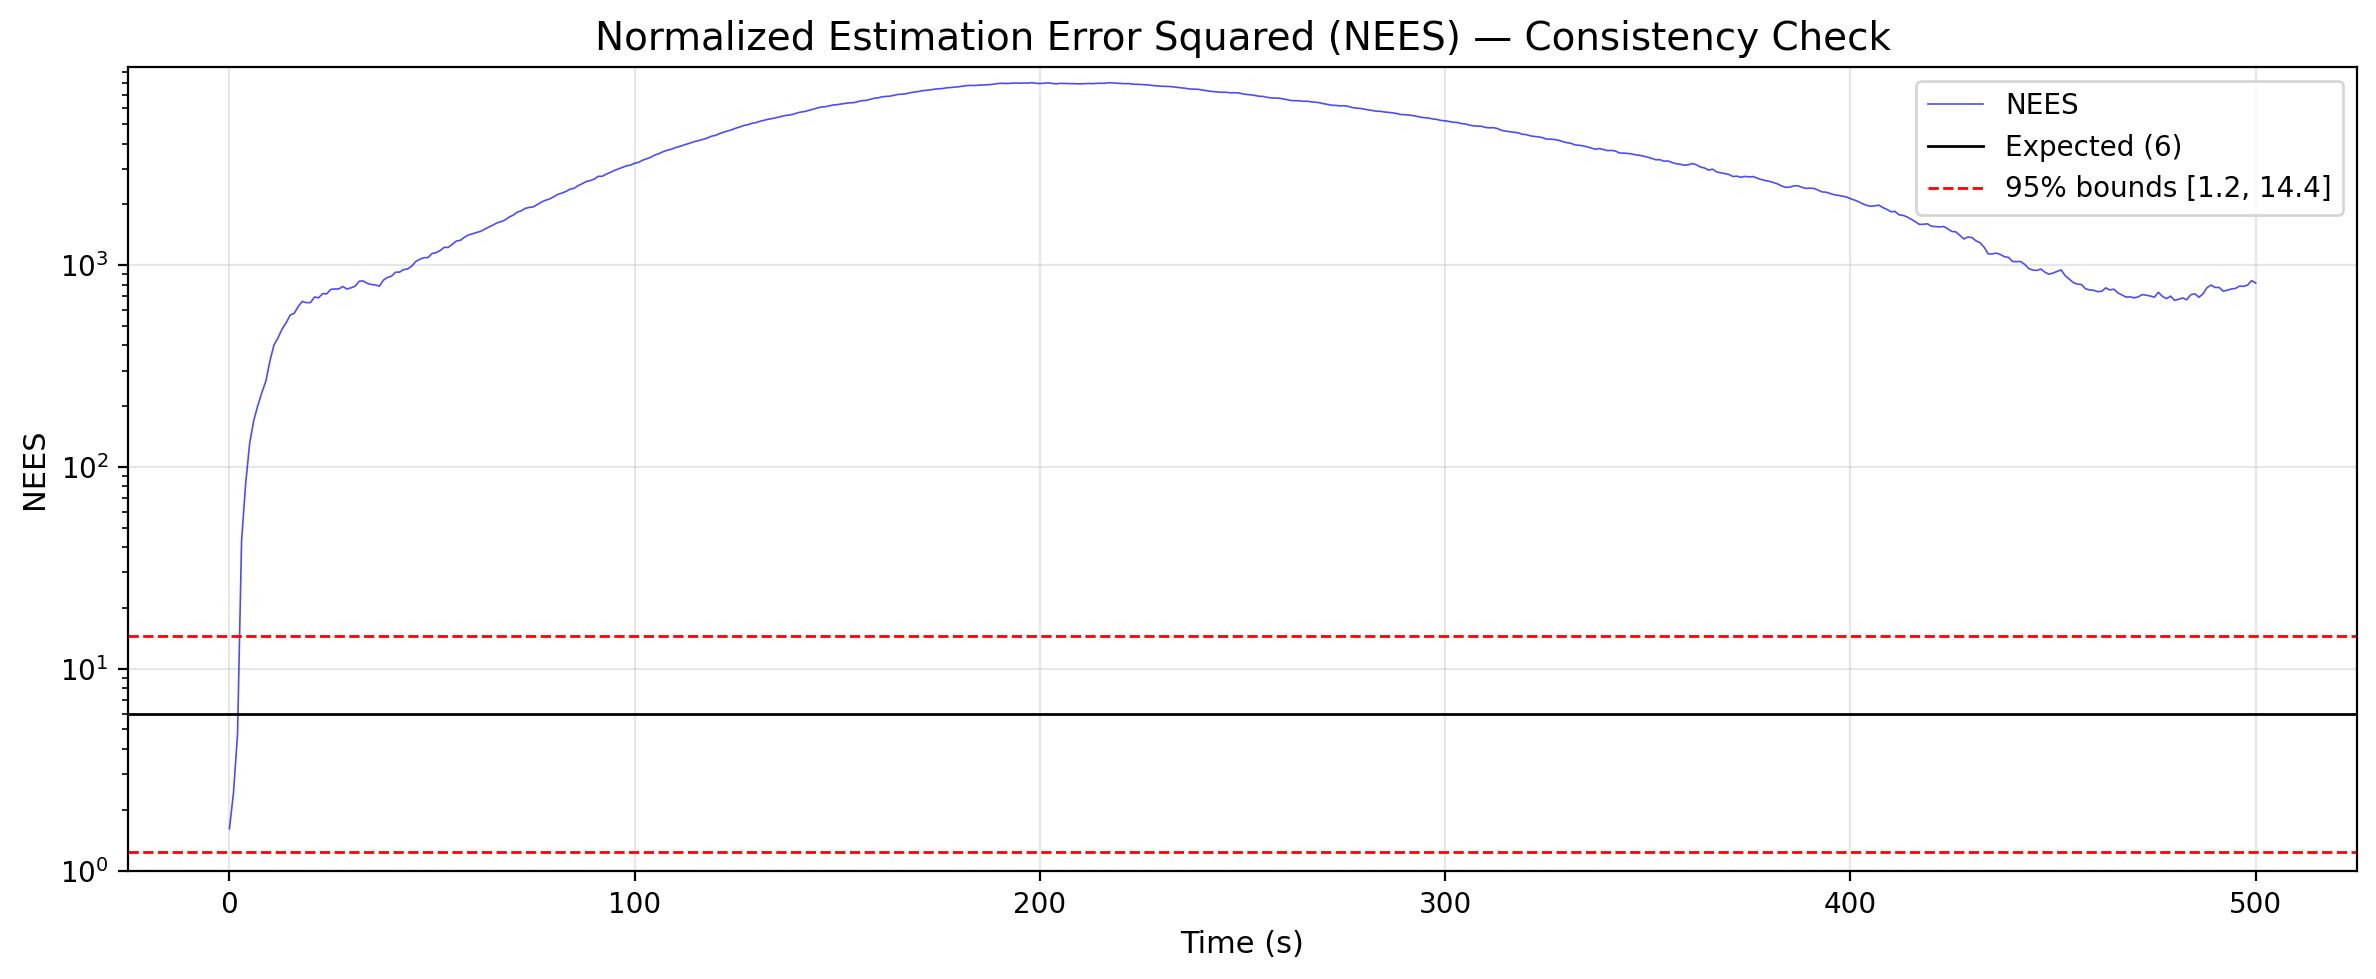
\includegraphics[width=\columnwidth]{mekf_nees.png}
  \caption{NEES consistency check.  The NEES exceeds the 95\% $\chi^2(6)$
    bounds by two to three orders of magnitude, indicating the filter is
    still strongly overconfident despite the corrected propagation model.}
  \label{fig:nees}
\end{figure}

The NEES remains far above the $\chi^2$ bounds: peak NEES is
$\sim$$8.0\times10^3$, the mean after 50~s is
$\sim$$4.1\times10^3$, and the final value is still $\sim$$8.2\times10^2$.
Thus the frame-rate bug was not the only issue; the estimator remains
severely overconfident.  The dominant causes are the unmodeled affine
sensor residuals and coarse one-step propagation error, both of which are
absorbed imperfectly by the current $Q$ and $R$ choices.  In practice, this
would be addressed by:
(1) augmenting the state with sensor calibration parameters,
(2) inflating process/measurement noise to account for unmodeled effects, or
(3) employing an adaptive filter that tunes $Q$ online.

\subsubsection{Convergence Behavior}

Fig.~\ref{fig:convergence} shows convergence from five initial attitude
errors ranging from 1$^\circ$ to 60$^\circ$.

\begin{figure}[t]
  \centering
  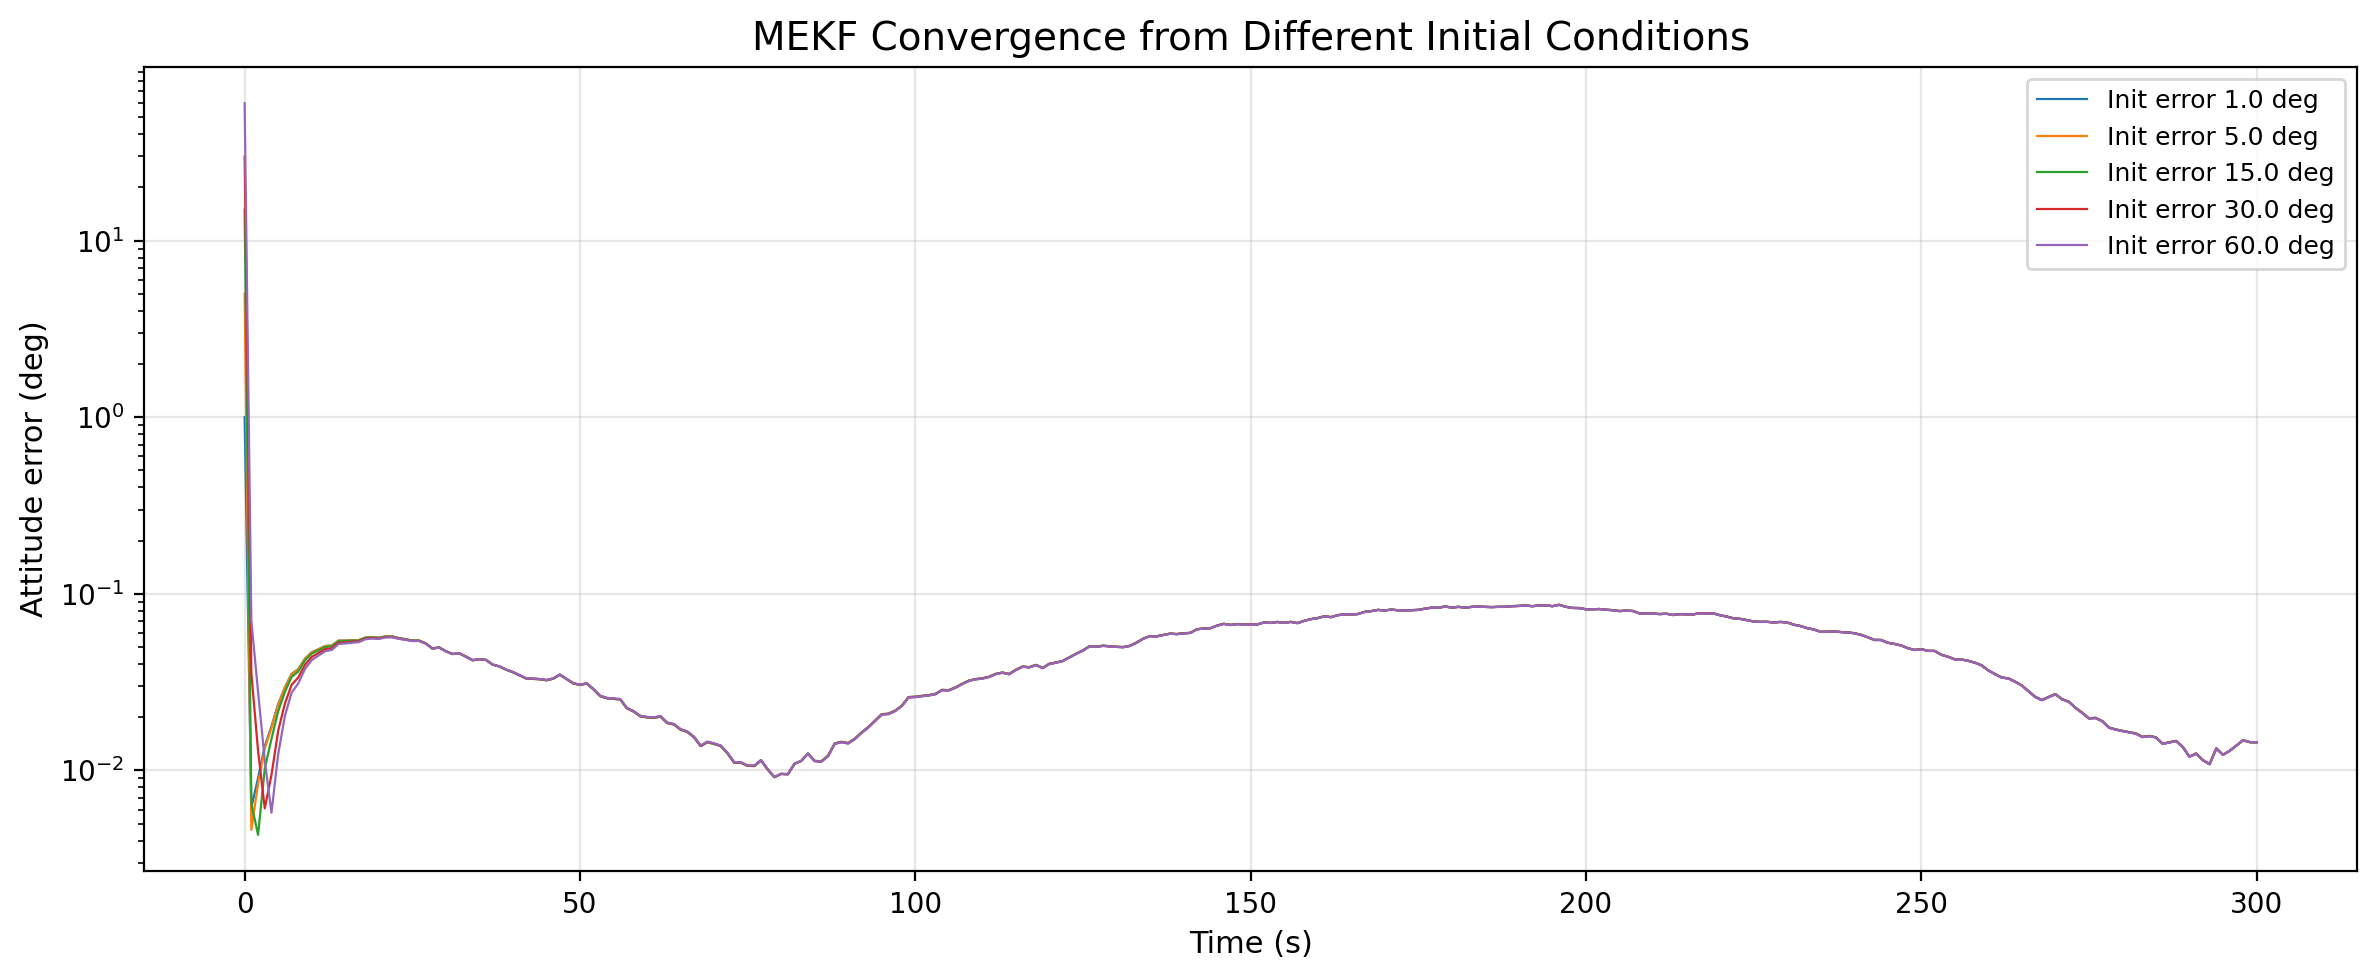
\includegraphics[width=\columnwidth]{mekf_convergence.png}
  \caption{MEKF convergence from different initial conditions.  The filter
    converges from all tested initial errors (1--60$^\circ$) within
    $\sim$50~s.  Steady-state accuracy is $\sim$0.025$^\circ$ regardless
    of initial error magnitude.}
  \label{fig:convergence}
\end{figure}

All cases converge within $\sim$50 seconds to steady-state accuracy of
$\sim$0.025$^\circ$.  Even from a 60$^\circ$ initial error, the MEKF
converges rapidly thanks to the star tracker quaternion update, which
provides a global attitude reference.  The convergence time is
approximately 3--5$\times$ the measurement update interval, consistent
with the filter's information gain per step.

\begin{figure}[t]
  \centering
  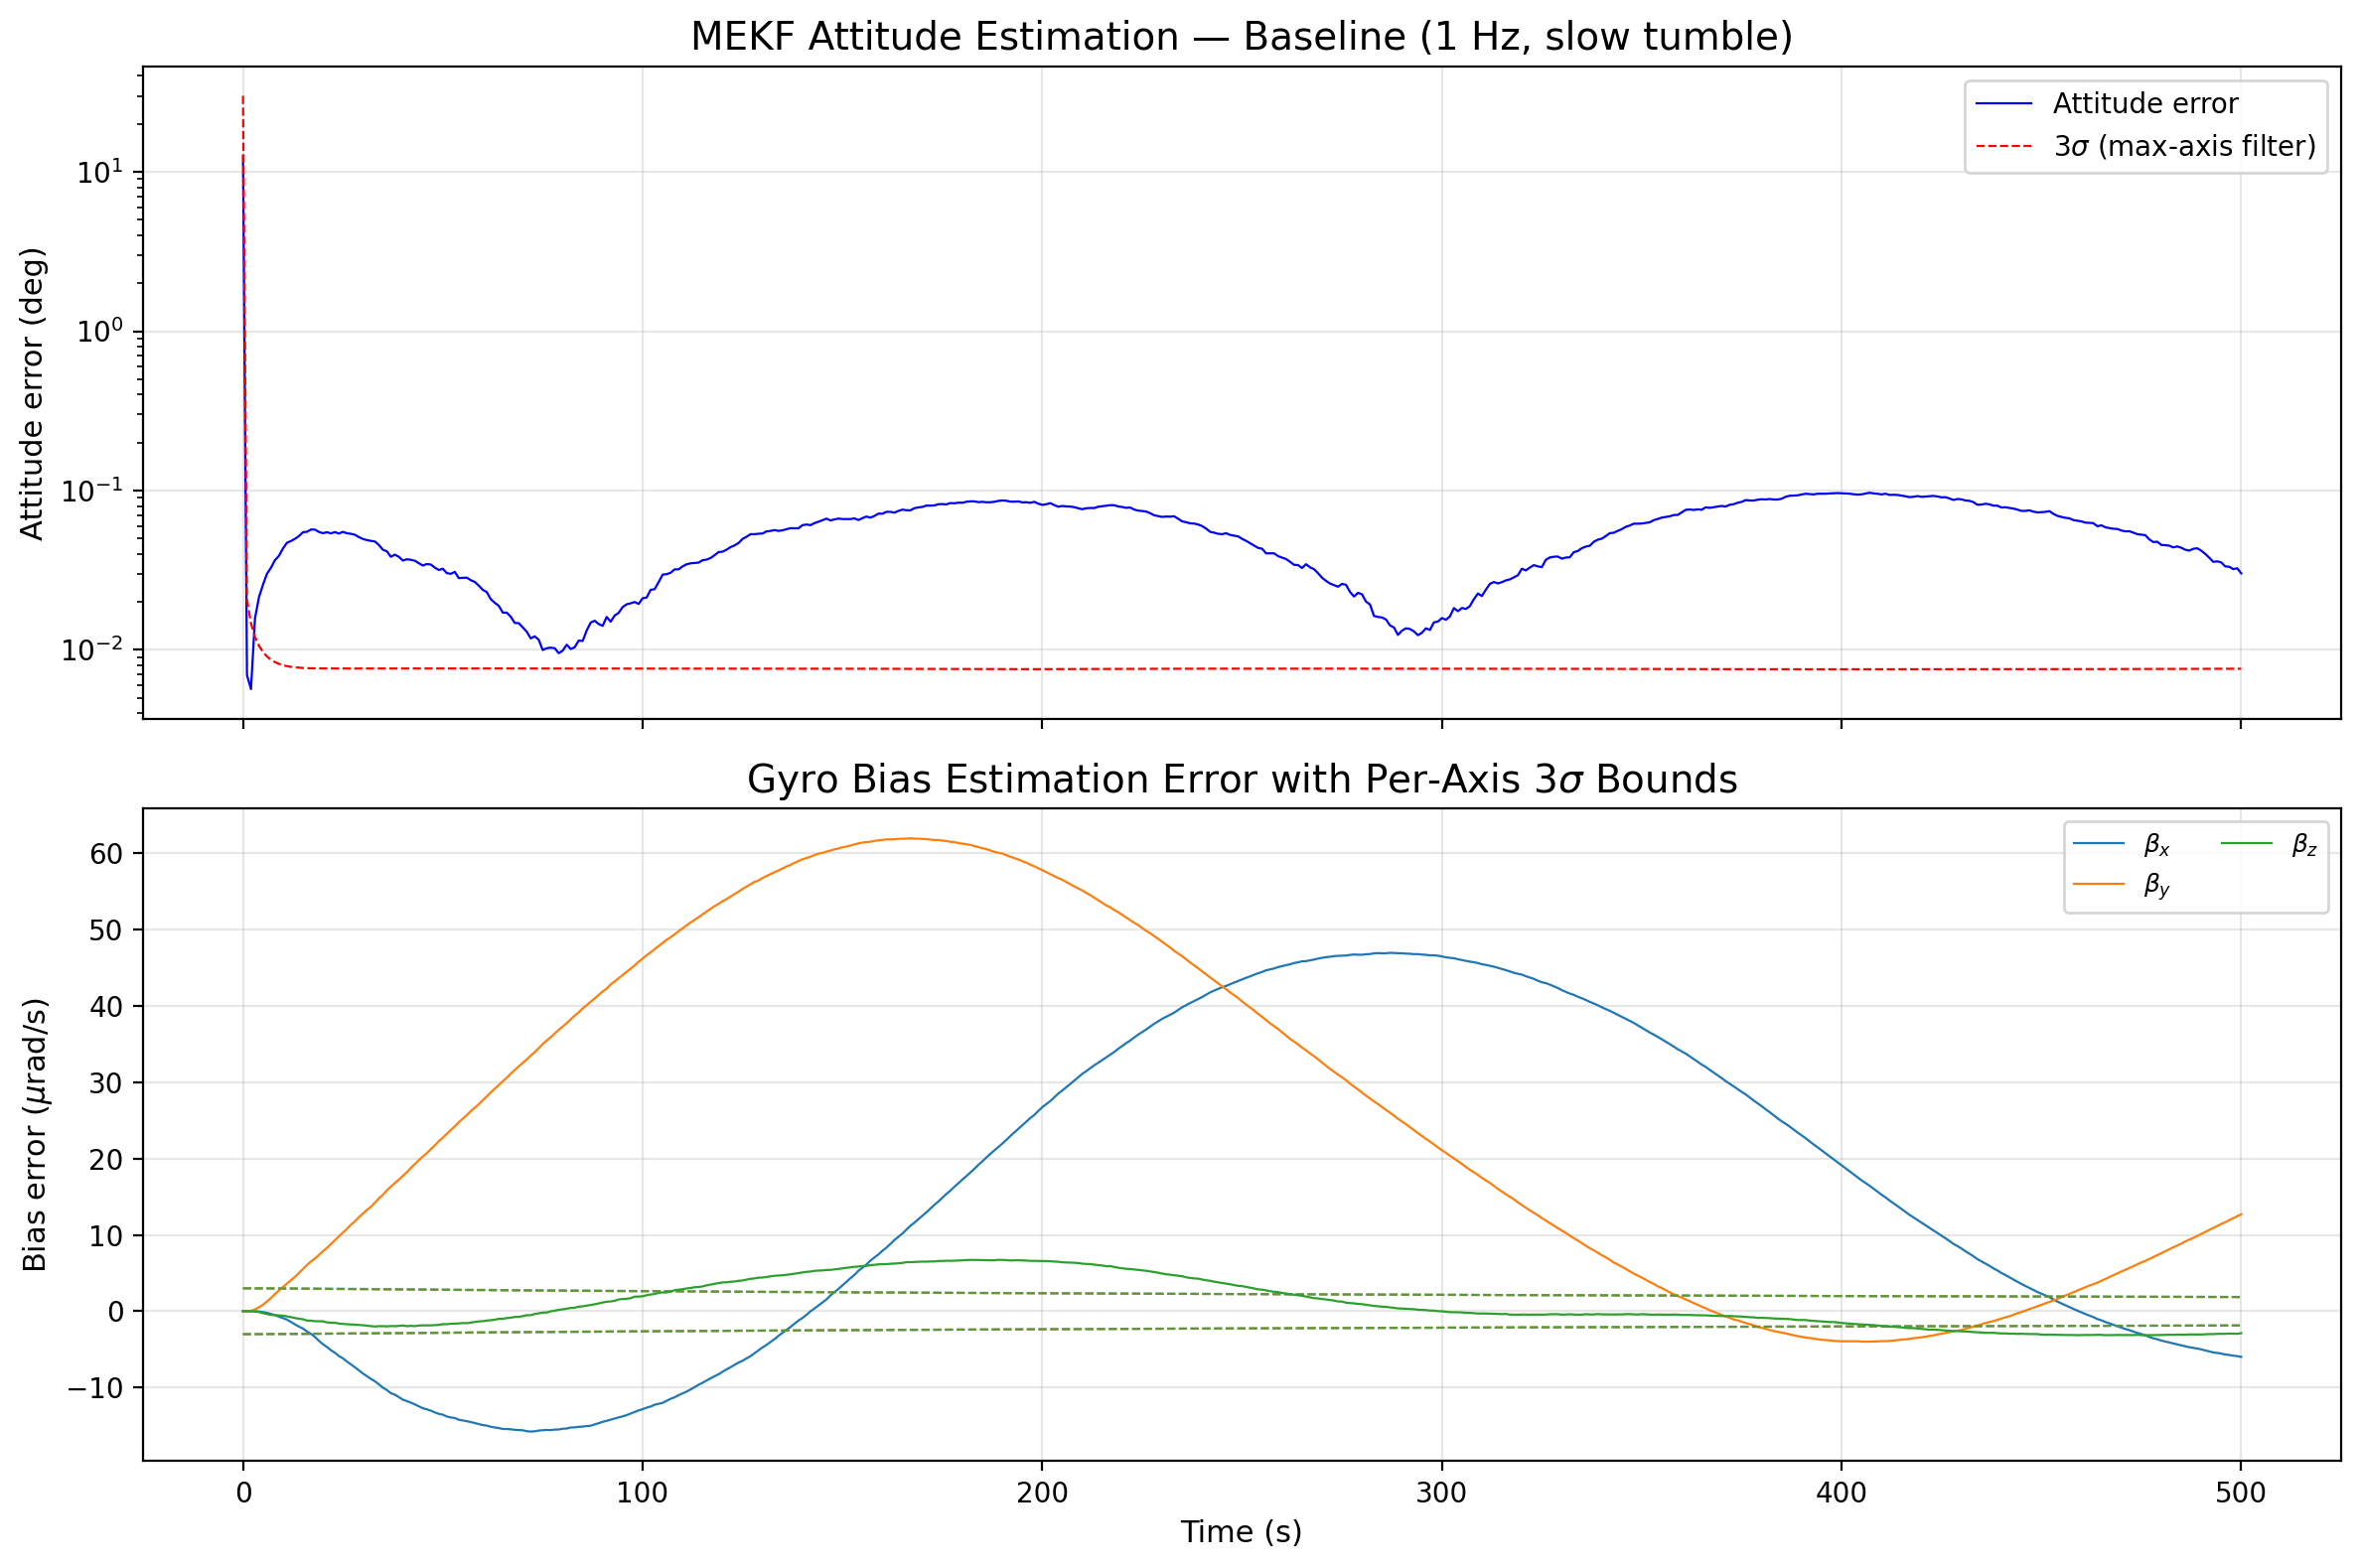
\includegraphics[width=\columnwidth]{mekf_baseline.png}
  \caption{Baseline MEKF performance at 1 Hz.  Top: attitude error
    (blue) with a conservative $3\sigma$ covariance proxy based on the
    largest attitude-covariance eigenvalue (red dashed).  The estimator
    converges within $\sim$30 s and maintains $\sim$0.05$^\circ$ accuracy,
    but the error still lies above the bound, confirming overconfidence.
    Bottom: gyro bias estimation error per axis with matching per-axis
    $3\sigma$ bounds.}
  \label{fig:baseline}
\end{figure}

The initial covariance $P_0$ should be set conservatively (i.e., larger
than the expected initial error) to ensure the filter accepts early
measurements.  Setting $P_0$ too small causes the filter to reject
informative measurements, delaying convergence.

% ------------------------------------------------------------------
\section{Changelog}

\begin{table}[h]
\centering
\begin{tabular}{@{}ll@{}}
\toprule
\textbf{Date} & \textbf{Description} \\
\midrule
2026-04-02 & HW3: Sensor models revisited, MEKF implementation \\
2026-03-12 & HW2: Safe mode, dynamics, sensors, estimation \\
2026-02-26 & HW1: Mission description, model, dynamics, Euler \\
\bottomrule
\end{tabular}
\end{table}

\begin{thebibliography}{9}
\bibitem{markley2014}
F.~L.~Markley and J.~L.~Crassidis,
\textit{Fundamentals of Spacecraft Attitude Determination and Control}.
New York: Springer, 2014.

\bibitem{lefferts1982}
E.~J.~Lefferts, F.~L.~Markley, and M.~D.~Shuster,
``Kalman filtering for spacecraft attitude estimation,''
\textit{J.~Guidance, Control, and Dynamics}, vol.~5, no.~5, pp.~417--429, 1982.

\bibitem{gg1320}
Honeywell, ``GG1320AN Digital Ring Laser Gyroscope,'' datasheet, 2020.

\bibitem{sodern}
Sodern, ``SED36 Star Tracker,'' product specification, 2019.

\bibitem{adcole}
Adcole Corporation, ``Two-Axis Digital Sun Sensor,'' datasheet.

\bibitem{hmc2003}
Honeywell, ``HMC2003 Three-Axis Magnetic Sensor Hybrid,'' datasheet, 2018.

\bibitem{smad}
J.~R.~Wertz and W.~J.~Larson,
\textit{Space Mission Analysis and Design}, 3rd ed.
Microcosm Press, 1999.

\bibitem{titterton}
D.~H.~Titterton and J.~L.~Weston,
\textit{Strapdown Inertial Navigation Technology}, 2nd ed.
IET, 2004.

\bibitem{nasa_iss}
NASA, ``International Space Station: Facts and Figures,''
\url{https://www.nasa.gov/feature/facts-and-figures}, 2024.
\end{thebibliography}

\end{document}
